\documentclass[aspectratio=169]{beamer}
\usepackage{amsmath}
\usepackage{amssymb}
\usepackage{xcolor}
\usepackage{tikz}
\usetikzlibrary{positioning}

% ================================================================
% Quick Questions deck: index rules.
%
% Each topic opens with five true/false statements and then runs ten
% quick questions that get gradually harder. Every question gets two
% slides: the question on its own for the mini whiteboards, then the
% same question again with the solution underneath in red.
%
% The three green topics work on the index laws themselves, first with
% positive indices, then with negative ones, then applied to algebraic
% expressions. The four amber topics move on to roots: estimating them,
% then indices of the form 1/a and a/b, and finally negative
% fractional indices.
%
% Where the working can be drawn it is: a halving ladder for the
% negative indices, number lines for the estimating, area and volume
% pictures for the square and cube roots, and flow charts for the
% fractional indices, which show the root, the power and the
% reciprocal as separate steps done in order.
% ================================================================

\setbeamertemplate{navigation symbols}{}

% A link in the bottom left of every slide back to the contents, so a
% deck this long can be jumped around in during a lesson.
\setbeamertemplate{footline}{%
  \hbox to\paperwidth{%
    \hspace{1em}%
    \hyperlink{contents}{%
      \color{gray}\scriptsize$\leftarrow$~Back to contents}%
    \hfil}%
  \vskip4pt%
}

% Topic divider.
\newcommand{\qtopic}[1]{%
  \section{#1}%
  \begin{frame}
    \vfill
    \begin{center}
      {\usebeamercolor[fg]{structure}\Huge\bfseries #1}
    \end{center}
    \vfill
  \end{frame}%
}

% \qq[<question size>][<solution size>]{<question>}{<solution>}
% The two optional sizes drop the type for the wordier questions and
% the longer solutions, so nothing runs off the slide.
\NewDocumentCommand{\qq}{O{\Huge}O{\LARGE}+m+m}{%
  \begin{frame}
    \vfill
    \begin{center}
      \begin{minipage}{0.92\textwidth}
        \centering #1 #3
      \end{minipage}
    \end{center}
    \vfill
  \end{frame}%
  \begin{frame}
    \vfill
    \begin{center}
      \begin{minipage}{0.92\textwidth}
        \centering #1 #3
        \par\vspace{0.9em}
        {\color{red}#2 #4}
      \end{minipage}
    \end{center}
    \vfill
  \end{frame}%
}

% \tf[<statement size>][<answer size>]{<statement>}{<answer>}
% As \qq, but with a standing "True or false?" heading above the
% statement. The statements hunt for the usual misconceptions, so the
% answer always says why, not just which.
\NewDocumentCommand{\tf}{O{\LARGE}O{\Large}+m+m}{%
  \begin{frame}
    \vfill
    \begin{center}
      \begin{minipage}{0.92\textwidth}
        \centering
        {\usebeamercolor[fg]{structure}\Large\bfseries True or false?}
        \par\vspace{1em}
        #1 #3
      \end{minipage}
    \end{center}
    \vfill
  \end{frame}%
  \begin{frame}
    \vfill
    \begin{center}
      \begin{minipage}{0.92\textwidth}
        \centering
        {\usebeamercolor[fg]{structure}\Large\bfseries True or false?}
        \par\vspace{1em}
        #1 #3
        \par\vspace{0.9em}
        {\color{red}#2 #4}
      \end{minipage}
    \end{center}
    \vfill
  \end{frame}%
}

% Chained working, one equation per row, so that a long run of index
% laws does not have to be squeezed onto a single line.
\newcommand{\work}[1]{%
  \begin{tabular}{@{}r@{\;=\;}l@{}}#1\end{tabular}%
}

% \flow{<start>}{<first step>}{<middle>}{<second step>}{<end>}
% A flow chart of three boxes joined by two labelled arrows. Used for
% the fractional indices, where the point is that the root and the
% power are separate steps, done one after the other.
\newcommand{\flow}[5]{%
  \begin{tikzpicture}[
      fbox/.style={draw=red!60!black, rounded corners=2pt, fill=red!8,
                   inner sep=5pt, text=red, font=\large},
      farr/.style={->, red, thick, shorten >=1pt, shorten <=1pt}]
    \node[fbox] (a) {$#1$};
    \node[fbox, right=2.4cm of a] (b) {$#3$};
    \node[fbox, right=2.4cm of b] (c) {$#5$};
    \draw[farr] (a) -- node[above,text=red,font=\small]{#2} (b);
    \draw[farr] (b) -- node[above,text=red,font=\small]{#4} (c);
  \end{tikzpicture}%
}

% \flowfour{<start>}{<step>}{<second>}{<step>}{<third>}{<step>}{<end>}
% The same chart with a third arrow, for the negative fractional
% indices, where taking the reciprocal is a step of its own.
\newcommand{\flowfour}[7]{%
  \begin{tikzpicture}[
      fbox/.style={draw=red!60!black, rounded corners=2pt, fill=red!8,
                   inner sep=4pt, text=red, font=\large},
      farr/.style={->, red, thick, shorten >=1pt, shorten <=1pt}]
    \node[fbox] (a) {$#1$};
    \node[fbox, right=2.0cm of a] (b) {$#3$};
    \node[fbox, right=2.0cm of b] (c) {$#5$};
    \node[fbox, right=2.0cm of c] (d) {$#7$};
    \draw[farr] (a) -- node[above,text=red,font=\small]{#2} (b);
    \draw[farr] (b) -- node[above,text=red,font=\small]{#4} (c);
    \draw[farr] (c) -- node[above,text=red,font=\small]{#6} (d);
  \end{tikzpicture}%
}

% The powers of 2 running down from 2^3 to 2^{-3}, halving at every
% step. The negative indices are not a new rule: they are the same
% pattern carried on past 2^0=1.
\newcommand{\halvingladder}{%
  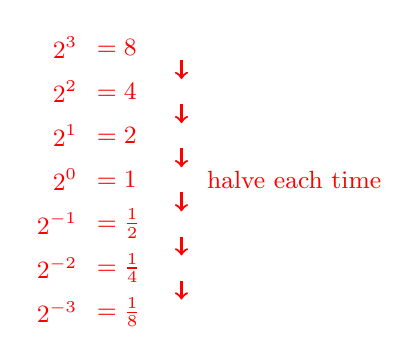
\begin{tikzpicture}[x=1cm,y=1cm,color=red,font=\small]
    \node[anchor=east] at (0,0)    {$2^{3}$};  \node[anchor=west] at (0,0)    {$=8$};
    \node[anchor=east] at (0,-0.56) {$2^{2}$};  \node[anchor=west] at (0,-0.56) {$=4$};
    \node[anchor=east] at (0,-1.12) {$2^{1}$};  \node[anchor=west] at (0,-1.12) {$=2$};
    \node[anchor=east] at (0,-1.68) {$2^{0}$};  \node[anchor=west] at (0,-1.68) {$=1$};
    \node[anchor=east] at (0,-2.24) {$2^{-1}$}; \node[anchor=west] at (0,-2.24) {$=\tfrac{1}{2}$};
    \node[anchor=east] at (0,-2.80) {$2^{-2}$}; \node[anchor=west] at (0,-2.80) {$=\tfrac{1}{4}$};
    \node[anchor=east] at (0,-3.36) {$2^{-3}$}; \node[anchor=west] at (0,-3.36) {$=\tfrac{1}{8}$};
    \foreach \i in {0,...,5}{%
      \draw[->,red,thick] (1.2,{-0.56*\i-0.16}) -- (1.2,{-0.56*\i-0.40});}
    \node[anchor=west,font=\small] at (1.4,-1.68) {halve each time};
  \end{tikzpicture}%
}

% \rootline{<left label>}{<right label>}{<root being estimated>}{<how far along, 0 to 1>}
% A number line running between the two whole numbers either side of a
% root, with the root marked in its true position between them.
\newcommand{\rootline}[4]{%
  \begin{tikzpicture}[x=1cm,y=1cm]
    \draw[red!55!black,thick] (0,0) -- (9,0);
    \draw[red!55!black,thick] (0,-0.16) -- (0,0.16);
    \draw[red!55!black,thick] (9,-0.16) -- (9,0.16);
    \node[red!55!black,below=6pt,font=\small] at (0,0) {$#1$};
    \node[red!55!black,below=6pt,font=\small] at (9,0) {$#2$};
    \fill[red] ({9*#4},0) circle (2.6pt);
    \node[red,above=5pt,font=\small] at ({9*#4},0) {$#3$};
  \end{tikzpicture}%
}

% \areasquare{<side>}{<area>} — a square labelled with its area and the
% side length that gives it. The square root of a number is the side of
% the square with that area, which is what the picture is there to say.
\newcommand{\areasquare}[2]{%
  \begin{tikzpicture}[x=1cm,y=1cm]
    \draw[red!60!black,thick,fill=red!8] (0,0) rectangle (2.4,2.4);
    \node[red,font=\small] at (1.2,1.2) {area $#2$};
    \node[red,font=\small,below=2pt] at (1.2,0) {$#1$};
    \node[red,font=\small,left=2pt] at (0,1.2) {$#1$};
  \end{tikzpicture}%
}

% \volumecube{<edge>}{<volume>} — the matching picture for cube roots:
% the cube root of a number is the edge of the cube with that volume.
\newcommand{\volumecube}[2]{%
  \begin{tikzpicture}[x=1cm,y=1cm]
    \draw[red!60!black,thick,fill=red!8] (0,0) rectangle (2,2);
    \draw[red!60!black,thick] (0,2) -- (0.7,2.7) -- (2.7,2.7) -- (2,2);
    \draw[red!60!black,thick] (2.7,2.7) -- (2.7,0.7) -- (2,0);
    \node[red,font=\small] at (1,1) {vol. $#2$};
    \node[red,font=\small,below=2pt] at (1,0) {$#1$};
  \end{tikzpicture}%
}

% Contents-slide bullets, colour-coded by difficulty band: green for
% the three index-law topics, orange for the four root topics. The
% green is darkened because a pure green washes out on a projector.
\setbeamertemplate{section in toc}{%
  \ifnum\inserttocsectionnumber<4
    \textcolor{green!55!black}{$\bullet$}%
  \else
    \textcolor{orange}{$\bullet$}%
  \fi
  ~\inserttocsection%
}

\title{Index Rules: Quick Questions}
\subtitle{Mini whiteboard questions, with solutions}
\author{}
\date{}

\begin{document}

\frame{\titlepage}

\begin{frame}[label=contents]{Contents}
  \small
  \tableofcontents
\end{frame}

%================================================================
\qtopic{Index rules with positive indices}
%================================================================

\tf{$4^{3}$ means $4\times 4\times 4$}
  {\textbf{True.} The index counts how many $4$s are multiplied
   together, so $4^{3}=64$.}

\tf{$2^{5}\times 2^{3}=2^{8}$}
  {\textbf{True.} Five $2$s multiplied by three $2$s gives eight $2$s,
   so the indices are added.}

\tf{$2^{5}\times 2^{3}=4^{8}$}
  {\textbf{False.} Only the indices are added; the base stays as $2$.\\[0.3em]
   The answer is $2^{8}=256$, not $4^{8}=65\,536$.}

\tf{$\dfrac{7^{8}}{7^{2}}=7^{4}$}
  {\textbf{False.} The indices are subtracted, not divided.\\[0.3em]
   $7^{8}\div 7^{2}=7^{8-2}=7^{6}$}

\tf{$\left(5^{2}\right)^{3}=5^{5}$}
  {\textbf{False.} $\left(5^{2}\right)^{3}=5^{2}\times 5^{2}\times 5^{2}$,
   which is six $5$s.\\[0.3em]
   The indices are multiplied: $5^{6}$.}

\qq[\Huge][\large]{Simplify $2^{3}\times 2^{4}$}
  {$(2\times 2\times 2)\times(2\times 2\times 2\times 2)$ --- seven $2$s
   \par\vspace{0.4em}
   $2^{3}\times 2^{4}=2^{3+4}=2^{7}$}

\qq{Simplify $5^{6}\div 5^{2}$}
  {$5^{6-2}=5^{4}$}

\qq{Simplify $7^{5}\times 7$}
  {$7$ on its own is $7^{1}$.\\[0.3em]
   $7^{5+1}=7^{6}$}

\qq{Simplify $\left(3^{2}\right)^{4}$}
  {$3^{2\times 4}=3^{8}$}

\qq{Simplify $4^{3}\times 4^{2}\times 4^{5}$}
  {$4^{3+2+5}=4^{10}$}

\qq[\Huge][\LARGE]{Simplify $\dfrac{6^{8}}{6^{3}\times 6^{2}}$}
  {\work{$6^{3}\times 6^{2}$ & $6^{5}$\\[0.3em]
         $\dfrac{6^{8}}{6^{5}}$ & $6^{8-5}=6^{3}$}}

\qq[\Huge][\LARGE]{Simplify $\left(2^{3}\right)^{2}\times 2^{4}$}
  {\work{$\left(2^{3}\right)^{2}$ & $2^{6}$\\[0.3em]
         $2^{6}\times 2^{4}$ & $2^{10}$}}

\qq[\Huge][\LARGE]{Simplify $\dfrac{\left(5^{3}\right)^{4}}{5^{10}}$}
  {\work{$\left(5^{3}\right)^{4}$ & $5^{12}$\\[0.3em]
         $\dfrac{5^{12}}{5^{10}}$ & $5^{12-10}=5^{2}$}}

\qq[\LARGE][\LARGE]{$3^{n}\times 3^{5}=3^{12}$\\[0.4em]Find the value of $n$}
  {The indices add, so $n+5=12$.\\[0.3em]
   $n=7$}

\qq[\LARGE][\LARGE]{Write $8^{4}$ as a power of $2$}
  {$8=2^{3}$, so $8^{4}=\left(2^{3}\right)^{4}$.\\[0.3em]
   $8^{4}=2^{12}$}

%================================================================
\qtopic{Index rules with negative indices}
%================================================================

\tf[\Large][\normalsize]{$2^{-3}$ is a negative number}
  {\textbf{False.} A negative index gives a reciprocal, not a negative answer.\\[0.3em]
   $2^{-3}=\dfrac{1}{2^{3}}=\dfrac{1}{8}$, which is positive.
   \par\vspace{0.4em}
   \halvingladder}

\tf{$5^{-1}=\dfrac{1}{5}$}
  {\textbf{True.} An index of $-1$ gives the reciprocal of the base.}

\tf{$4^{-2}=\dfrac{1}{8}$}
  {\textbf{False.} The $-2$ is an index, not a multiplier.\\[0.3em]
   $4^{-2}=\dfrac{1}{4^{2}}=\dfrac{1}{16}$}

\tf{$2^{4}\div 2^{7}=2^{-3}$}
  {\textbf{True.} The indices are subtracted: $4-7=-3$.}

\tf{$2^{-3}\times 2^{5}=2^{-15}$}
  {\textbf{False.} The indices are added, not multiplied.\\[0.3em]
   $2^{-3+5}=2^{2}=4$}

\qq[\Huge][\large]{Write $2^{-1}$ as a fraction}
  {$2^{-1}=\dfrac{1}{2}$
   \par\vspace{0.5em}
   \halvingladder}

\qq{Write $3^{-2}$ as a fraction}
  {$3^{-2}=\dfrac{1}{3^{2}}=\dfrac{1}{9}$}

\qq[\Huge][\LARGE]{Write $\dfrac{1}{5^{3}}$ using a negative index}
  {$\dfrac{1}{5^{3}}=5^{-3}$}

\qq[\LARGE][\LARGE]{Write $10^{-3}$ as a decimal}
  {$10^{-3}=\dfrac{1}{10^{3}}=\dfrac{1}{1000}=0.001$}

\qq{Simplify $2^{3}\times 2^{-5}$}
  {$2^{3+(-5)}=2^{-2}$}

\qq{Simplify $7^{-2}\div 7^{3}$}
  {$7^{-2-3}=7^{-5}$}

\qq{Simplify $\left(4^{-2}\right)^{3}$}
  {$4^{-2\times 3}=4^{-6}$}

\qq[\Huge][\LARGE]{Work out $\dfrac{5^{-3}}{5^{-7}}$}
  {\work{$5^{-3-(-7)}$ & $5^{-3+7}$\\[0.3em]
         $5^{4}$ & $625$}}

\qq[\Huge][\LARGE]{Work out $\left(\dfrac{2}{3}\right)^{-2}$}
  {A negative index gives the reciprocal of the fraction.\\[0.4em]
   $\left(\dfrac{3}{2}\right)^{2}=\dfrac{9}{4}$}

\qq[\LARGE][\LARGE]{$2^{n}\times 2^{-5}=2^{-1}$\\[0.4em]Find the value of $n$}
  {The indices add, so $n-5=-1$.\\[0.3em]
   $n=4$}

%================================================================
\qtopic{Simplifying expressions with index laws}
%================================================================

\tf{$x^{3}\times x^{4}=x^{12}$}
  {\textbf{False.} The indices are added, not multiplied.\\[0.3em]
   $x^{3}\times x^{4}=x^{7}$}

\tf{$2a^{3}\times 3a^{2}=6a^{5}$}
  {\textbf{True.} The numbers are multiplied and the indices are added.}

\tf{$\left(2x^{3}\right)^{2}=2x^{6}$}
  {\textbf{False.} Everything inside the bracket is squared, including
   the $2$.\\[0.3em]
   $\left(2x^{3}\right)^{2}=2^{2}\times x^{6}=4x^{6}$}

\tf{$x^{5}+x^{3}=x^{8}$}
  {\textbf{False.} Indices are added when terms are multiplied, not
   when they are added.\\[0.3em]
   $x^{5}+x^{3}$ cannot be simplified.}

\tf{$\dfrac{12x^{5}}{3x^{5}}=4$}
  {\textbf{True.} $12\div 3=4$ and $x^{5}\div x^{5}=x^{0}=1$.}

\qq{Simplify $x^{3}\times x^{4}$}
  {$x^{3+4}=x^{7}$}

\qq{Simplify $y^{8}\div y^{3}$}
  {$y^{8-3}=y^{5}$}

\qq{Simplify $3a^{2}\times 4a^{5}$}
  {$3\times 4=12$ and $a^{2+5}=a^{7}$\\[0.3em]
   $12a^{7}$}

\qq[\Huge][\LARGE]{Simplify $\dfrac{20b^{7}}{5b^{2}}$}
  {$20\div 5=4$ and $b^{7-2}=b^{5}$\\[0.3em]
   $4b^{5}$}

\qq{Simplify $\left(x^{4}\right)^{3}$}
  {$x^{4\times 3}=x^{12}$}

\qq[\Huge][\LARGE]{Simplify $\left(3m^{2}\right)^{3}$}
  {The $3$ is cubed as well as the $m^{2}$.\\[0.3em]
   $3^{3}\times m^{6}=27m^{6}$}

\qq[\LARGE][\LARGE]{Simplify $5p^{3}q^{2}\times 4p^{2}q^{5}$}
  {$5\times 4=20$, $p^{3+2}=p^{5}$, $q^{2+5}=q^{7}$\\[0.3em]
   $20p^{5}q^{7}$}

\qq[\LARGE][\LARGE]{Simplify $\dfrac{18x^{6}y^{4}}{6x^{2}y^{4}}$}
  {$18\div 6=3$, $x^{6-2}=x^{4}$, $y^{4-4}=y^{0}=1$\\[0.3em]
   $3x^{4}$}

\qq[\LARGE][\LARGE]{Simplify $\dfrac{\left(2x^{3}\right)^{4}}{8x^{5}}$}
  {\work{$\left(2x^{3}\right)^{4}$ & $16x^{12}$\\[0.3em]
         $\dfrac{16x^{12}}{8x^{5}}$ & $2x^{7}$}}

\qq[\Large][\LARGE]{Simplify $\dfrac{6a^{5}b^{2}\times 3a^{2}b^{4}}{9a^{4}b^{3}}$}
  {\work{$6a^{5}b^{2}\times 3a^{2}b^{4}$ & $18a^{7}b^{6}$\\[0.3em]
         $\dfrac{18a^{7}b^{6}}{9a^{4}b^{3}}$ & $2a^{3}b^{3}$}}

%================================================================
\qtopic{Estimating roots and powers}
%================================================================

\tf[\LARGE][\large]{$\sqrt{50}$ lies between $7$ and $8$}
  {\textbf{True.} $7^{2}=49$ and $8^{2}=64$, and $50$ lies between
   those two square numbers.
   \par\vspace{0.6em}
   \rootline{\sqrt{49}=7}{\sqrt{64}=8}{\sqrt{50}}{0.071}}

\tf{$\sqrt{20}=10$}
  {\textbf{False.} Square rooting is not halving.\\[0.3em]
   $10^{2}=100$, not $20$. In fact $\sqrt{20}$ is between $4$ and $5$.}

\tf{$\sqrt{1000}$ is about $100$}
  {\textbf{False.} $100^{2}=10\,000$, not $1000$.\\[0.3em]
   $31^{2}=961$ and $32^{2}=1024$, so $\sqrt{1000}$ is about $31.6$.}

\tf[\LARGE][\large]{$\sqrt[3]{30}$ lies between $3$ and $4$}
  {\textbf{True.} $3^{3}=27$ and $4^{3}=64$, and $30$ lies between
   those two cube numbers.
   \par\vspace{0.6em}
   \rootline{\sqrt[3]{27}=3}{\sqrt[3]{64}=4}{\sqrt[3]{30}}{0.107}}

\tf{$\sqrt{0.64}$ is smaller than $0.64$}
  {\textbf{False.} Square rooting only makes a number smaller when it
   is bigger than $1$.\\[0.3em]
   $0.8^{2}=0.64$, so $\sqrt{0.64}=0.8$, which is larger than $0.64$.}

\qq[\Huge][\large]{Between which two whole numbers\\[0.3em]does $\sqrt{30}$ lie?}
  {Between $5$ and $6$, because $5^{2}=25$ and $6^{2}=36$.
   \par\vspace{0.6em}
   \rootline{\sqrt{25}=5}{\sqrt{36}=6}{\sqrt{30}}{0.477}}

\qq[\Huge][\large]{Between which two whole numbers\\[0.3em]does $\sqrt{75}$ lie?}
  {Between $8$ and $9$, because $8^{2}=64$ and $9^{2}=81$.
   \par\vspace{0.6em}
   \rootline{\sqrt{64}=8}{\sqrt{81}=9}{\sqrt{75}}{0.660}}

\qq[\LARGE][\LARGE]{Estimate $3.9^{3}$}
  {Round $3.9$ to $4$.\\[0.3em]
   $4^{3}=64$, so $3.9^{3}$ is about $64$.}

\qq[\Huge][\large]{Between which two whole numbers\\[0.3em]does $\sqrt[3]{50}$ lie?}
  {Between $3$ and $4$, because $3^{3}=27$ and $4^{3}=64$.
   \par\vspace{0.6em}
   \rootline{\sqrt[3]{27}=3}{\sqrt[3]{64}=4}{\sqrt[3]{50}}{0.684}}

\qq[\LARGE][\large]{Estimate $\sqrt{17}$\\[0.3em]to one decimal place}
  {$\sqrt{16}=4$, so the answer is just above $4$.\\[0.3em]
   $4.1^{2}=16.81$ and $4.2^{2}=17.64$, so $\sqrt{17}\approx 4.1$.}

\qq[\LARGE][\large]{Estimate $\sqrt{90}$\\[0.3em]to one decimal place}
  {$\sqrt{81}=9$ and $\sqrt{100}=10$, so the answer is between
   $9$ and $10$.\\[0.3em]
   $9.5^{2}=90.25$, so $\sqrt{90}\approx 9.5$.}

\qq[\LARGE][\LARGE]{Which is larger,\\[0.3em]$\sqrt{40}$ or $6.5$?}
  {Square both: $\left(\sqrt{40}\right)^{2}=40$ and $6.5^{2}=42.25$.\\[0.3em]
   $6.5$ is larger.}

\qq[\LARGE][\large]{Estimate $\sqrt{2000}$\\[0.3em]to the nearest whole number}
  {$44^{2}=1936$ and $45^{2}=2025$.\\[0.3em]
   $2000$ is nearer to $2025$, so $\sqrt{2000}\approx 45$.}

\qq[\LARGE][\LARGE]{Estimate $\dfrac{\sqrt{101}}{4.9}$}
  {Round each part: $\sqrt{101}\approx\sqrt{100}=10$ and $4.9\approx 5$.\\[0.3em]
   $\dfrac{10}{5}=2$}

\qq[\Large][\large]{A square patio has an area of $150\ \mathrm{m^{2}}$.\\[0.4em]
   Estimate the length of one side.}
  {The side is $\sqrt{150}$.\\[0.3em]
   $12^{2}=144$ and $13^{2}=169$, so the side is just over $12$.\\[0.3em]
   $12.2^{2}=148.84$, so the side is about $12.2\ \mathrm{m}$.}

%================================================================
\qtopic{Indices of the form \texorpdfstring{$\frac{1}{a}$}{1/a}}
%================================================================

\tf[\LARGE][\large]{$9^{\frac{1}{2}}=3$}
  {\textbf{True.} An index of $\frac{1}{2}$ means the square root, and
   $3^{2}=9$.
   \par\vspace{0.5em}
   \areasquare{3}{9}}

\tf{$9^{\frac{1}{2}}=4.5$}
  {\textbf{False.} The index is not a multiplier, so this is not half
   of $9$.\\[0.3em]
   $9^{\frac{1}{2}}=\sqrt{9}=3$}

\tf[\LARGE][\large]{$8^{\frac{1}{3}}=2$}
  {\textbf{True.} An index of $\frac{1}{3}$ means the cube root, and
   $2^{3}=8$.
   \par\vspace{0.5em}
   \volumecube{2}{8}}

\tf{$16^{\frac{1}{4}}=4$}
  {\textbf{False.} An index of $\frac{1}{4}$ means the fourth root, not
   the square root.\\[0.3em]
   $2^{4}=16$, so $16^{\frac{1}{4}}=2$. It is $16^{\frac{1}{2}}$ that
   equals $4$.}

\tf{$100^{\frac{1}{3}}=10$}
  {\textbf{False.} $10^{3}=1000$, not $100$.\\[0.3em]
   $\sqrt[3]{100}$ is about $4.6$. It is $100^{\frac{1}{2}}$ that
   equals $10$.}

\qq[\Huge][\large]{Work out $25^{\frac{1}{2}}$}
  {$25^{\frac{1}{2}}=\sqrt{25}=5$
   \par\vspace{0.5em}
   \areasquare{5}{25}}

\qq{Work out $64^{\frac{1}{2}}$}
  {$\sqrt{64}=8$, because $8^{2}=64$.}

\qq[\Huge][\large]{Work out $27^{\frac{1}{3}}$}
  {$\sqrt[3]{27}=3$, because $3^{3}=27$.
   \par\vspace{0.5em}
   \volumecube{3}{27}}

\qq[\Huge][\LARGE]{Work out $81^{\frac{1}{4}}$}
  {The fourth root: $3\times 3\times 3\times 3=81$.\\[0.3em]
   $81^{\frac{1}{4}}=3$}

\qq[\Huge][\LARGE]{Work out $1000^{\frac{1}{3}}$}
  {$\sqrt[3]{1000}=10$, because $10^{3}=1000$.}

\qq[\Huge][\LARGE]{Write $\sqrt[5]{x}$ using an index}
  {$\sqrt[5]{x}=x^{\frac{1}{5}}$}

\qq[\Huge][\LARGE]{Work out $\left(\dfrac{1}{16}\right)^{\frac{1}{2}}$}
  {Square root the numerator and the denominator.\\[0.3em]
   $\dfrac{\sqrt{1}}{\sqrt{16}}=\dfrac{1}{4}$}

\qq[\Huge][\LARGE]{Work out $\left(\dfrac{8}{27}\right)^{\frac{1}{3}}$}
  {Cube root the numerator and the denominator.\\[0.3em]
   $\dfrac{\sqrt[3]{8}}{\sqrt[3]{27}}=\dfrac{2}{3}$}

\qq[\Huge][\LARGE]{Work out $0.04^{\frac{1}{2}}$}
  {$0.2\times 0.2=0.04$\\[0.3em]
   $0.04^{\frac{1}{2}}=0.2$}

\qq[\Huge][\LARGE]{Work out $\left(\dfrac{1}{32}\right)^{\frac{1}{5}}$}
  {The fifth root of $32$ is $2$, because $2^{5}=32$.\\[0.3em]
   $\dfrac{1}{2}$}

%================================================================
\qtopic{Indices of the form \texorpdfstring{$\frac{a}{b}$}{a/b}}
%================================================================

\tf[\LARGE][\large]{$8^{\frac{2}{3}}=4$}
  {\textbf{True.} The denominator of the index gives the root and
   the numerator gives the power.
   \par\vspace{0.6em}
   \flow{8}{cube root}{2}{square it}{4}}

\tf[\LARGE][\large]{$16^{\frac{3}{4}}=12$}
  {\textbf{False.} This is $\frac{3}{4}$ of $16$, not $16$ to the power
   $\frac{3}{4}$.
   \par\vspace{0.6em}
   \flow{16}{fourth root}{2}{cube it}{8}}

\tf{$25^{\frac{3}{2}}=75$}
  {\textbf{False.} The $\frac{3}{2}$ is an index, not a multiplier.\\[0.3em]
   $\sqrt{25}=5$, then $5^{3}=125$.}

\tf[\LARGE][\large]{To work out $32^{\frac{3}{5}}$ you can find
   $\sqrt[5]{32}$ first,\\[0.3em]then cube the answer}
  {\textbf{True.} Finding the root first keeps the numbers small.
   \par\vspace{0.6em}
   \flow{32}{fifth root}{2}{cube it}{8}}

\tf{$4^{\frac{3}{2}}$ and $4^{1.5}$ mean the same thing}
  {\textbf{True.} $\frac{3}{2}=1.5$, so both are $\sqrt{4}$ cubed,
   which is $8$.}

\qq[\Huge][\large]{Work out $4^{\frac{3}{2}}$}
  {\flow{4}{square root}{2}{cube it}{8}}

\qq[\Huge][\large]{Work out $8^{\frac{2}{3}}$}
  {\flow{8}{cube root}{2}{square it}{4}}

\qq[\Huge][\large]{Work out $9^{\frac{3}{2}}$}
  {\flow{9}{square root}{3}{cube it}{27}}

\qq[\Huge][\large]{Work out $16^{\frac{3}{4}}$}
  {\flow{16}{fourth root}{2}{cube it}{8}}

\qq[\Huge][\large]{Work out $27^{\frac{2}{3}}$}
  {\flow{27}{cube root}{3}{square it}{9}}

\qq[\Huge][\large]{Work out $32^{\frac{3}{5}}$}
  {\flow{32}{fifth root}{2}{cube it}{8}}

\qq[\Huge][\large]{Work out $125^{\frac{4}{3}}$}
  {\flow{125}{cube root}{5}{fourth power}{625}}

\qq[\Huge][\LARGE]{Work out $\left(\dfrac{4}{9}\right)^{\frac{3}{2}}$}
  {\work{$\left(\dfrac{4}{9}\right)^{\frac{1}{2}}$ & $\dfrac{2}{3}$\\[0.6em]
         $\left(\dfrac{2}{3}\right)^{3}$ & $\dfrac{8}{27}$}}

\qq[\Huge][\LARGE]{Work out $0.25^{\frac{3}{2}}$}
  {$\sqrt{0.25}=0.5$, because $0.5^{2}=0.25$.\\[0.3em]
   $0.5^{3}=0.125$}

\qq[\Huge][\LARGE]{Work out $\left(\dfrac{16}{81}\right)^{\frac{3}{4}}$}
  {\work{$\left(\dfrac{16}{81}\right)^{\frac{1}{4}}$ & $\dfrac{2}{3}$\\[0.6em]
         $\left(\dfrac{2}{3}\right)^{3}$ & $\dfrac{8}{27}$}}

%================================================================
\qtopic{Simplifying expressions with negative fractional indices}
%================================================================

\tf[\LARGE][\large]{$9^{-\frac{1}{2}}=\dfrac{1}{3}$}
  {\textbf{True.} The $\frac{1}{2}$ gives the square root and the minus
   sign gives the reciprocal.
   \par\vspace{0.6em}
   \flow{9}{square root}{3}{reciprocal}{\tfrac{1}{3}}}

\tf{$9^{-\frac{1}{2}}=-3$}
  {\textbf{False.} A negative index gives a reciprocal, not a negative
   answer.\\[0.3em]
   $9^{-\frac{1}{2}}=\dfrac{1}{\sqrt{9}}=\dfrac{1}{3}$}

\tf[\LARGE][\large]{$8^{-\frac{2}{3}}=\dfrac{1}{4}$}
  {\textbf{True.} Cube root, then square, then take the reciprocal.
   \par\vspace{0.6em}
   \flowfour{8}{cube root}{2}{square it}{4}{reciprocal}{\tfrac{1}{4}}}

\tf{$16^{-\frac{3}{4}}=\dfrac{1}{12}$}
  {\textbf{False.} The $\frac{3}{4}$ is an index, not a multiplier.\\[0.3em]
   $\sqrt[4]{16}=2$, then $2^{3}=8$, so the answer is $\dfrac{1}{8}$.}

\tf[\LARGE][\large]{$25^{-\frac{1}{2}}$ is smaller than $25^{-\frac{3}{2}}$}
  {\textbf{False.} The more negative the index, the smaller the result
   for a base bigger than $1$.\\[0.3em]
   $25^{-\frac{1}{2}}=\dfrac{1}{5}=0.2$ and
   $25^{-\frac{3}{2}}=\dfrac{1}{125}=0.008$.}

\qq[\Huge][\LARGE]{Work out $4^{-\frac{1}{2}}$}
  {$4^{-\frac{1}{2}}=\dfrac{1}{\sqrt{4}}=\dfrac{1}{2}$}

\qq[\Huge][\LARGE]{Work out $8^{-\frac{1}{3}}$}
  {$8^{-\frac{1}{3}}=\dfrac{1}{\sqrt[3]{8}}=\dfrac{1}{2}$}

\qq[\Huge][\LARGE]{Work out $9^{-\frac{1}{2}}$}
  {$9^{-\frac{1}{2}}=\dfrac{1}{\sqrt{9}}=\dfrac{1}{3}$}

\qq[\Huge][\large]{Work out $27^{-\frac{2}{3}}$}
  {\flowfour{27}{cube root}{3}{square it}{9}{reciprocal}{\tfrac{1}{9}}}

\qq[\Huge][\large]{Work out $16^{-\frac{3}{4}}$}
  {\flowfour{16}{fourth root}{2}{cube it}{8}{reciprocal}{\tfrac{1}{8}}}

\qq[\Huge][\LARGE]{Work out $\left(\dfrac{1}{4}\right)^{-\frac{1}{2}}$}
  {Take the reciprocal of the fraction, then square root.\\[0.3em]
   $4^{\frac{1}{2}}=2$}

\qq[\Huge][\LARGE]{Work out $\left(\dfrac{9}{16}\right)^{-\frac{1}{2}}$}
  {Take the reciprocal of the fraction, then square root.\\[0.4em]
   $\left(\dfrac{16}{9}\right)^{\frac{1}{2}}=\dfrac{4}{3}$}

\qq[\Huge][\large]{Work out $\left(\dfrac{8}{27}\right)^{-\frac{2}{3}}$}
  {\work{$\left(\dfrac{8}{27}\right)^{-\frac{2}{3}}$ & $\left(\dfrac{27}{8}\right)^{\frac{2}{3}}$\\[0.6em]
         $\left(\dfrac{27}{8}\right)^{\frac{2}{3}}$ & $\left(\dfrac{3}{2}\right)^{2}$\\[0.6em]
         $\left(\dfrac{3}{2}\right)^{2}$ & $\dfrac{9}{4}$}}

\qq[\Huge][\LARGE]{Simplify $\dfrac{x^{\frac{1}{2}}}{x^{-\frac{3}{2}}}$}
  {The indices are subtracted.\\[0.3em]
   $x^{\frac{1}{2}-\left(-\frac{3}{2}\right)}=x^{2}$}

\qq[\LARGE][\LARGE]{Simplify $\left(16x^{8}\right)^{-\frac{3}{4}}$}
  {\work{$\left(16x^{8}\right)^{\frac{1}{4}}$ & $2x^{2}$\\[0.4em]
         $\left(2x^{2}\right)^{3}$ & $8x^{6}$\\[0.4em]
         $\left(16x^{8}\right)^{-\frac{3}{4}}$ & $\dfrac{1}{8x^{6}}$}}

\end{document}
